
%% bare_conf.tex
%% V1.3
%% 2007/01/11
%% by Michael Shell
%% See:
%% http://www.michaelshell.org/
%% for current contact information.
%%
%% This is a skeleton file demonstrating the use of IEEEtran.cls
%% (requires IEEEtran.cls version 1.7 or later) with an IEEE conference paper.
%%
%% Support sites:
%% http://www.michaelshell.org/tex/ieeetran/
%% http://www.ctan.org/tex-archive/macros/latex/contrib/IEEEtran/
%% and
%% http://www.ieee.org/

%%*************************************************************************
%% Legal Notice:
%% This code is offered as-is without any warranty either expressed or
%% implied; without even the implied warranty of MERCHANTABILITY or
%% FITNESS FOR A PARTICULAR PURPOSE!
%% User assumes all risk.
%% In no event shall IEEE or any contributor to this code be liable for
%% any damages or losses, including, but not limited to, incidental,
%% consequential, or any other damages, resulting from the use or misuse
%% of any information contained here.
%%
%% All comments are the opinions of their respective authors and are not
%% necessarily endorsed by the IEEE.
%%
%% This work is distributed under the LaTeX Project Public License (LPPL)
%% ( http://www.latex-project.org/ ) version 1.3, and may be freely used,
%% distributed and modified. A copy of the LPPL, version 1.3, is included
%% in the base LaTeX documentation of all distributions of LaTeX released
%% 2003/12/01 or later.
%% Retain all contribution notices and credits.
%% ** Modified files should be clearly indicated as such, including  **
%% ** renaming them and changing author support contact information. **
%%
%% File list of work: IEEEtran.cls, IEEEtran_HOWTO.pdf, bare_adv.tex,
%%                    bare_conf.tex, bare_jrnl.tex, bare_jrnl_compsoc.tex
%%*************************************************************************

% *** Authors should verify (and, if needed, correct) their LaTeX system  ***
% *** with the testflow diagnostic prior to trusting their LaTeX platform ***
% *** with production work. IEEE's font choices can trigger bugs that do  ***
% *** not appear when using other class files.                            ***
% The testflow support page is at:
% http://www.michaelshell.org/tex/testflow/



% Note that the a4paper option is mainly intended so that authors in
% countries using A4 can easily print to A4 and see how their papers will
% look in print - the typesetting of the document will not typically be
% affected with changes in paper size (but the bottom and side margins will).
% Use the testflow package mentioned above to verify correct handling of
% both paper sizes by the user's LaTeX system.
%
% Also note that the "draftcls" or "draftclsnofoot", not "draft", option
% should be used if it is desired that the figures are to be displayed in
% draft mode.
%
\documentclass[conference]{IEEEtran}
% Add the compsoc option for Computer Society conferences.
%
% If IEEEtran.cls has not been installed into the LaTeX system files,
% manually specify the path to it like:
% \documentclass[conference]{../sty/IEEEtran}





% Some very useful LaTeX packages include:
% (uncomment the ones you want to load)


% *** MISC UTILITY PACKAGES ***
%
%\usepackage{ifpdf}
% Heiko Oberdiek's ifpdf.sty is very useful if you need conditional
% compilation based on whether the output is pdf or dvi.
% usage:
% \ifpdf
%   % pdf code
% \else
%   % dvi code
% \fi
% The latest version of ifpdf.sty can be obtained from:
% http://www.ctan.org/tex-archive/macros/latex/contrib/oberdiek/
% Also, note that IEEEtran.cls V1.7 and later provides a builtin
% \ifCLASSINFOpdf conditional that works the same way.
% When switching from latex to pdflatex and vice-versa, the compiler may
% have to be run twice to clear warning/error messages.






% *** CITATION PACKAGES ***
%
%\usepackage{cite}
% cite.sty was written by Donald Arseneau
% V1.6 and later of IEEEtran pre-defines the format of the cite.sty package
% \cite{} output to follow that of IEEE. Loading the cite package will
% result in citation numbers being automatically sorted and properly
% "compressed/ranged". e.g., [1], [9], [2], [7], [5], [6] without using
% cite.sty will become [1], [2], [5]--[7], [9] using cite.sty. cite.sty's
% \cite will automatically add leading space, if needed. Use cite.sty's
% noadjust option (cite.sty V3.8 and later) if you want to turn this off.
% cite.sty is already installed on most LaTeX systems. Be sure and use
% version 4.0 (2003-05-27) and later if using hyperref.sty. cite.sty does
% not currently provide for hyperlinked citations.
% The latest version can be obtained at:
% http://www.ctan.org/tex-archive/macros/latex/contrib/cite/
% The documentation is contained in the cite.sty file itself.






% *** GRAPHICS RELATED PACKAGES ***
%
\ifCLASSINFOpdf
  % \usepackage[pdftex]{graphicx}
  % declare the path(s) where your graphic files are
  % \graphicspath{{../pdf/}{../jpeg/}}
  % and their extensions so you won't have to specify these with
  % every instance of \includegraphics
  % \DeclareGraphicsExtensions{.pdf,.jpeg,.png}
\else
  % or other class option (dvipsone, dvipdf, if not using dvips). graphicx
  % will default to the driver specified in the system graphics.cfg if no
  % driver is specified.
  % \usepackage[dvips]{graphicx}
  % declare the path(s) where your graphic files are
  % \graphicspath{{../eps/}}
  % and their extensions so you won't have to specify these with
  % every instance of \includegraphics
  % \DeclareGraphicsExtensions{.eps}
\fi
% graphicx was written by David Carlisle and Sebastian Rahtz. It is
% required if you want graphics, photos, etc. graphicx.sty is already
% installed on most LaTeX systems. The latest version and documentation can
% be obtained at:
% http://www.ctan.org/tex-archive/macros/latex/required/graphics/
% Another good source of documentation is "Using Imported Graphics in
% LaTeX2e" by Keith Reckdahl which can be found as epslatex.ps or
% epslatex.pdf at: http://www.ctan.org/tex-archive/info/
%
% latex, and pdflatex in dvi mode, support graphics in encapsulated
% postscript (.eps) format. pdflatex in pdf mode supports graphics
% in .pdf, .jpeg, .png and .mps (metapost) formats. Users should ensure
% that all non-photo figures use a vector format (.eps, .pdf, .mps) and
% not a bitmapped formats (.jpeg, .png). IEEE frowns on bitmapped formats
% which can result in "jaggedy"/blurry rendering of lines and letters as
% well as large increases in file sizes.
%
% You can find documentation about the pdfTeX application at:
% http://www.tug.org/applications/pdftex

\usepackage[dvips]{graphicx}
\DeclareGraphicsExtensions{.eps}



% *** MATH PACKAGES ***
%
%\usepackage[cmex10]{amsmath}
% A popular package from the American Mathematical Society that provides
% many useful and powerful commands for dealing with mathematics. If using
% it, be sure to load this package with the cmex10 option to ensure that
% only type 1 fonts will utilized at all point sizes. Without this option,
% it is possible that some math symbols, particularly those within
% footnotes, will be rendered in bitmap form which will result in a
% document that can not be IEEE Xplore compliant!
%
% Also, note that the amsmath package sets \interdisplaylinepenalty to 10000
% thus preventing page breaks from occurring within multiline equations. Use:
%\interdisplaylinepenalty=2500
% after loading amsmath to restore such page breaks as IEEEtran.cls normally
% does. amsmath.sty is already installed on most LaTeX systems. The latest
% version and documentation can be obtained at:
% http://www.ctan.org/tex-archive/macros/latex/required/amslatex/math/





% *** SPECIALIZED LIST PACKAGES ***
%
%\usepackage{algorithmic}
% algorithmic.sty was written by Peter Williams and Rogerio Brito.
% This package provides an algorithmic environment fo describing algorithms.
% You can use the algorithmic environment in-text or within a figure
% environment to provide for a floating algorithm. Do NOT use the algorithm
% floating environment provided by algorithm.sty (by the same authors) or
% algorithm2e.sty (by Christophe Fiorio) as IEEE does not use dedicated
% algorithm float types and packages that provide these will not provide
% correct IEEE style captions. The latest version and documentation of
% algorithmic.sty can be obtained at:
% http://www.ctan.org/tex-archive/macros/latex/contrib/algorithms/
% There is also a support site at:
% http://algorithms.berlios.de/index.html
% Also of interest may be the (relatively newer and more customizable)
% algorithmicx.sty package by Szasz Janos:
% http://www.ctan.org/tex-archive/macros/latex/contrib/algorithmicx/




% *** ALIGNMENT PACKAGES ***
%
%\usepackage{array}
% Frank Mittelbach's and David Carlisle's array.sty patches and improves
% the standard LaTeX2e array and tabular environments to provide better
% appearance and additional user controls. As the default LaTeX2e table
% generation code is lacking to the point of almost being broken with
% respect to the quality of the end results, all users are strongly
% advised to use an enhanced (at the very least that provided by array.sty)
% set of table tools. array.sty is already installed on most systems. The
% latest version and documentation can be obtained at:
% http://www.ctan.org/tex-archive/macros/latex/required/tools/


%\usepackage{mdwmath}
%\usepackage{mdwtab}
% Also highly recommended is Mark Wooding's extremely powerful MDW tools,
% especially mdwmath.sty and mdwtab.sty which are used to format equations
% and tables, respectively. The MDWtools set is already installed on most
% LaTeX systems. The lastest version and documentation is available at:
% http://www.ctan.org/tex-archive/macros/latex/contrib/mdwtools/


% IEEEtran contains the IEEEeqnarray family of commands that can be used to
% generate multiline equations as well as matrices, tables, etc., of high
% quality.


%\usepackage{eqparbox}
% Also of notable interest is Scott Pakin's eqparbox package for creating
% (automatically sized) equal width boxes - aka "natural width parboxes".
% Available at:
% http://www.ctan.org/tex-archive/macros/latex/contrib/eqparbox/





% *** SUBFIGURE PACKAGES ***
\usepackage[tight,footnotesize]{subfigure}
% subfigure.sty was written by Steven Douglas Cochran. This package makes it
% easy to put subfigures in your figures. e.g., "Figure 1a and 1b". For IEEE
% work, it is a good idea to load it with the tight package option to reduce
% the amount of white space around the subfigures. subfigure.sty is already
% installed on most LaTeX systems. The latest version and documentation can
% be obtained at:
% http://www.ctan.org/tex-archive/obsolete/macros/latex/contrib/subfigure/
% subfigure.sty has been superceeded by subfig.sty.



%\usepackage[caption=false]{caption}
%\usepackage[font=footnotesize]{subfig}
% subfig.sty, also written by Steven Douglas Cochran, is the modern
% replacement for subfigure.sty. However, subfig.sty requires and
% automatically loads Axel Sommerfeldt's caption.sty which will override
% IEEEtran.cls handling of captions and this will result in nonIEEE style
% figure/table captions. To prevent this problem, be sure and preload
% caption.sty with its "caption=false" package option. This is will preserve
% IEEEtran.cls handing of captions. Version 1.3 (2005/06/28) and later
% (recommended due to many improvements over 1.2) of subfig.sty supports
% the caption=false option directly:
%\usepackage[caption=false,font=footnotesize]{subfig}
%
% The latest version and documentation can be obtained at:
% http://www.ctan.org/tex-archive/macros/latex/contrib/subfig/
% The latest version and documentation of caption.sty can be obtained at:
% http://www.ctan.org/tex-archive/macros/latex/contrib/caption/




% *** FLOAT PACKAGES ***
%
%\usepackage{fixltx2e}
% fixltx2e, the successor to the earlier fix2col.sty, was written by
% Frank Mittelbach and David Carlisle. This package corrects a few problems
% in the LaTeX2e kernel, the most notable of which is that in current
% LaTeX2e releases, the ordering of single and double column floats is not
% guaranteed to be preserved. Thus, an unpatched LaTeX2e can allow a
% single column figure to be placed prior to an earlier double column
% figure. The latest version and documentation can be found at:
% http://www.ctan.org/tex-archive/macros/latex/base/



%\usepackage{stfloats}
% stfloats.sty was written by Sigitas Tolusis. This package gives LaTeX2e
% the ability to do double column floats at the bottom of the page as well
% as the top. (e.g., "\begin{figure*}[!b]" is not normally possible in
% LaTeX2e). It also provides a command:
%\fnbelowfloat
% to enable the placement of footnotes below bottom floats (the standard
% LaTeX2e kernel puts them above bottom floats). This is an invasive package
% which rewrites many portions of the LaTeX2e float routines. It may not work
% with other packages that modify the LaTeX2e float routines. The latest
% version and documentation can be obtained at:
% http://www.ctan.org/tex-archive/macros/latex/contrib/sttools/
% Documentation is contained in the stfloats.sty comments as well as in the
% presfull.pdf file. Do not use the stfloats baselinefloat ability as IEEE
% does not allow \baselineskip to stretch. Authors submitting work to the
% IEEE should note that IEEE rarely uses double column equations and
% that authors should try to avoid such use. Do not be tempted to use the
% cuted.sty or midfloat.sty packages (also by Sigitas Tolusis) as IEEE does
% not format its papers in such ways.





% *** PDF, URL AND HYPERLINK PACKAGES ***
%
%\usepackage{url}
% url.sty was written by Donald Arseneau. It provides better support for
% handling and breaking URLs. url.sty is already installed on most LaTeX
% systems. The latest version can be obtained at:
% http://www.ctan.org/tex-archive/macros/latex/contrib/misc/
% Read the url.sty source comments for usage information. Basically,
% \url{my_url_here}.





% *** Do not adjust lengths that control margins, column widths, etc. ***
% *** Do not use packages that alter fonts (such as pslatex).         ***
% There should be no need to do such things with IEEEtran.cls V1.6 and later.
% (Unless specifically asked to do so by the journal or conference you plan
% to submit to, of course. )


% correct bad hyphenation here
\hyphenation{op-tical net-works semi-conduc-tor}


\begin{document}
%
% paper title
% can use linebreaks \\ within to get better formatting as desired
\title{Using Generalized Query Tree to cope with the Capture Effect in RFID Singulation}


% author names and affiliations
% use a multiple column layout for up to three different
% affiliations
\author{\IEEEauthorblockN{Victor K. Y. Wu}
\IEEEauthorblockA{Department of Electrical and Computer Engineering\\
University of Illinois at Urbana-Champaign, Illinois\\
Email: vwu3@illinois.edu}
\and
\IEEEauthorblockN{Roy H. Campbell}
\IEEEauthorblockA{Department of Computer Science\\
University of Illinois at Urbana-Champaign, Illinois\\
Email: rhc@illinois.edu}}

% conference papers do not typically use \thanks and this command
% is locked out in conference mode. If really needed, such as for
% the acknowledgment of grants, issue a \IEEEoverridecommandlockouts
% after \documentclass

% for over three affiliations, or if they all won't fit within the width
% of the page, use this alternative format:
%
%\author{\IEEEauthorblockN{Michael Shell\IEEEauthorrefmark{1},
%Homer Simpson\IEEEauthorrefmark{2},
%James Kirk\IEEEauthorrefmark{3},
%Montgomery Scott\IEEEauthorrefmark{3} and
%Eldon Tyrell\IEEEauthorrefmark{4}}
%\IEEEauthorblockA{\IEEEauthorrefmark{1}School of Electrical and Computer Engineering\\
%Georgia Institute of Technology,
%Atlanta, Georgia 30332--0250\\ Email: see http://www.michaelshell.org/contact.html}
%\IEEEauthorblockA{\IEEEauthorrefmark{2}Twentieth Century Fox, Springfield, USA\\
%Email: homer@thesimpsons.com}
%\IEEEauthorblockA{\IEEEauthorrefmark{3}Starfleet Academy, San Francisco, California 96678-2391\\
%Telephone: (800) 555--1212, Fax: (888) 555--1212}
%\IEEEauthorblockA{\IEEEauthorrefmark{4}Tyrell Inc., 123 Replicant Street, Los Angeles, California 90210--4321}}




% use for special paper notices
%\IEEEspecialpapernotice{(Invited Paper)}




% make the title area
\maketitle


\begin{abstract}
%\boldmath
The Query Tree Protocol (QT) in \cite{conf:Law01} is an efficient RFID tag singulation algorithm that is guaranteed to read all the tags in the broadcast range of a reader.  However, QT ignores the \em capture effect\em.  That is, after the reader broadcasts a bit string query prefix, it is assumed that it can distinguish one of three responses, namely \{no response, one response, collision\}.  If the capture effect is modeled, QT would no longer be guaranteed to singulate all the tags in the reader's range, since ``capturing'' a tag ID in the midst of a collision would leave all the other tags in that collision unsingulated.  In this paper, we introduce two modifications to QT that always singulate all the tags even when the capture effect is considered.  We call these the \em Generalized Query Tree Protocols \em (GQT1, GQT2).  We provide analytical bounds and simulation results of the singulation times of these new protocols in relation to QT.
\end{abstract}
% IEEEtran.cls defaults to using nonbold math in the Abstract.
% This preserves the distinction between vectors and scalars. However,
% if the conference you are submitting to favors bold math in the abstract,
% then you can use LaTeX's standard command \boldmath at the very start
% of the abstract to achieve this. Many IEEE journals/conferences frown on
% math in the abstract anyway.

% no keywords




% For peer review papers, you can put extra information on the cover
% page as needed:
% \ifCLASSOPTIONpeerreview
% \begin{center} \bfseries EDICS Category: 3-BBND \end{center}
% \fi
%
% For peerreview papers, this IEEEtran command inserts a page break and
% creates the second title. It will be ignored for other modes.
\IEEEpeerreviewmaketitle

% no \IEEEPARstart
\section{Introduction}
Radio frequency identification (RFID) passive tag singulation is the process where a single reader collects the identifiers (IDs) of all the passive tags in its broadcast range.  Since the tags share the same wireless medium for backscattering, singulation algorithms are collision resolution protocols.  There are two main classes of such protocols.  In probabilistic approaches, a mechanism similar to Aloha is used, where the reader broadcasts a query, telling each tag to randomly choose a time slot in which to reply \cite{conf:Vogt01}.  A collision occurs when two or more tags choose the same time slot.  In contrast, the Query Tree Protocol (QT) in \cite{conf:Law01} is a deterministic approach.  In this case, the reader successively sends longer query prefixes.  If a tag's ID matches the prefix, the tag responds with it's entire ID.  A collision occurs when two or more tags' IDs match the same prefix.  Since the query prefixes become longer, eventually only one tag will respond.  \cite{conf:Chiang01}, \cite{conf:Bhandari01}, and \cite{journal:Myung01} provide improvements to QT, but they are all based on the same underlying principle.

In \cite{conf:Law01}, after the reader broadcasts a bit string query prefix, it is assumed that it can distinguish one of three responses, namely \{no response, one response, collision\}.  In other words, the capture effect, which is a receiver decoding a signal even in the presence of other interfering signals, is ignored.  If the capture effect is modeled, QT would no longer be guaranteed to singulate all the tags in the reader's range, since ``capturing'' a tag ID in the midst of a collision would leave all the other tags in that collision unsingulated.  In this paper, we introduce two modifications to QT that always singulate all the tags even when the capture effect is considered.  We call these the \em Generalized Query Tree Protocols \em (GQT1, GQT2).  An important performance metric for these protocols is the time required to singulate all the tags.  We provide analytical bounds and simulation results on the singulation times of GQT1 and GQT2, and compare them to QT.

The rest of the paper is organized as follows.  In Section \ref{sec:model}, we provide the system model for tag singulation.  In Section \ref{sec:qt}, we re-introduce QT as explained in \cite{conf:Law01}, and explain its shortcomings in the context of the capture effect.  In Section \ref{sec:gqt}, we introduce our new protocols, GQT1, and GQT2.  In Section \ref{sec:sims}, we provide simulation results.  Section \ref{sec:con} concludes the paper.

\section{System Model}
\label{sec:model}
\begin{figure}
\centering
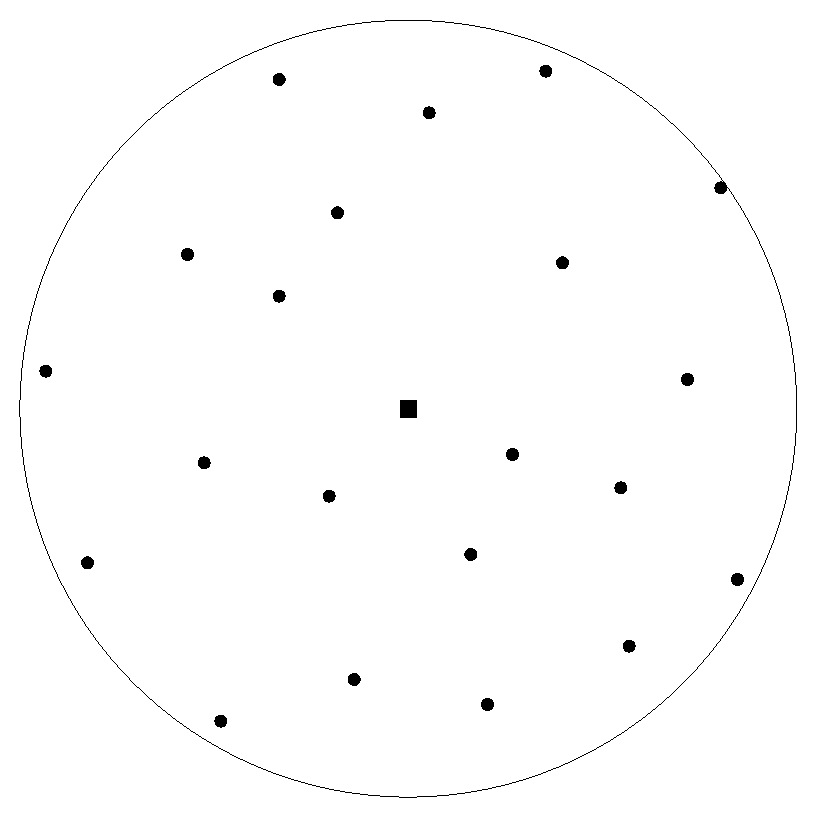
\includegraphics[width=1.5in]{fig1.eps}
\caption{Tag singulation on a circular disk of unit radius.  The tags are indicated by the small circles.  The reader is indicated by the square, which is located at the center of the disk.\label{fig:fig1}}
\end{figure}
We introduce the system model for tag singulation.  A single reader is located at the center of a circular disk of unit radius, which represents the transmit range of the reader.  That is, any tag lying in the disk can decode the reader's transmissions.  $n$ tags are placed in the disk, with their locations following a uniform distribution.  This is shown in Fig. \ref{fig:fig1}.  Each tag has a unique binary string identifier (ID) of length $k$ bits.  Therefore, $n \leq 2^k$.  The $n$ IDs are chosen uniformly.

Using a wireless transmission protocol, the reader and the tags work together, in order for the reader to collect all the tag IDs.  The reader has a single antenna, and transmits signals in an omni-directional fashion.  The reader also has no a priori knowledge of $n$.  The tags are passive.  That is, they transmit by backscattering energy received by the reader's transmissions.

\section{Query Tree Protocol}
\label{sec:qt}
In this section, we consider the Query Tree Protocol (QT), as explained in \cite{conf:Law01}.  The algorithm works with the reader repeatedly sending a query, and then waiting for a response from the tags.  In each query, the reader asks the tags if their IDs contain a certain prefix.  All the tags that do, respond by sending their tag IDs.  If more than one tag responds, the reader detects a collision.  It then appends a 0 or 1 to the prefix, and makes another query with the new longer prefix.  When only one tag responds, its ID can be decoded by the reader.  Each query prefix is associated with a node in a full binary tree (the query tree).  If a node has prefix xxx, then its two children have prefixes xxx0 and xxx1.  Fig. \ref{fig:fig2}, reproduced from \cite{conf:Law01}, illustrates QT.  Note that \cite{conf:Law01} does not take into account of the locations of the tags, as we model in Section \ref{sec:model}.  That is, the backscattered signals of the responding tags for a particular query are assumed to be received simultaneously at the reader.  The algorithm is shown below for completeness and comparison.  At the end of the algorithm, the IDs of all the tags are stored in $M$.
\begin{figure}
\centering
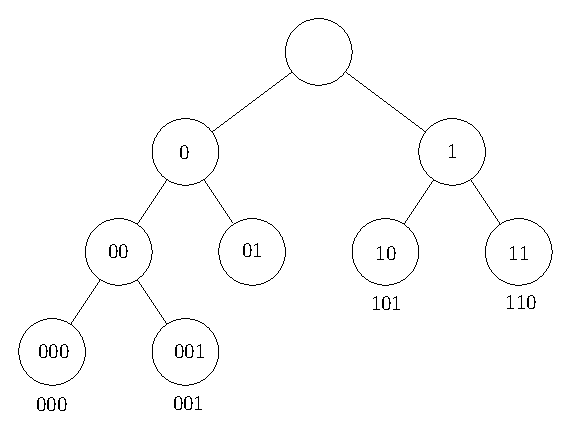
\includegraphics[width=2in]{fig2.eps}
\caption{QT with tag IDs \{000, 001, 101, 110\}.  The bit strings inside each node are query prefixes.  In a query prefix that results in one tag responding, the associated node is a leaf, and the bit string below that leaf is the decoded tag ID.  Note that the query prefix $01$ is also associated with a leaf, but since it results in no response from the tags, there is no ID below it.  \label{fig:fig2}}
\end{figure}
\begin{quote}
\em QT Protocol \em \\
\begin{footnotesize}
\textbf{Reader}
\begin{enumerate}
\item $Q:=\langle0,1\rangle$, and $M:=\langle \rangle$.
\item Suppose $Q = \langle q_1, \ldots, q_l \rangle$, and \\$M = \langle t_1, \ldots, t_m\rangle$.
\item Broadcast query $q_1$ to tags.   $Q := \langle q_2, \ldots, q_l \rangle$.
\item Listen to responses from tags.
\begin{itemize}
\item If no response, then do nothing.
\item Else if the response is tag ID $t$, then \\$M := \langle t_1, \ldots, t_m, t\rangle$.
\item Else, a collision is detected, then \\$Q := \langle q_2, \ldots, q_l, q_10, q_11 \rangle$.
\end{itemize}
\item If $Q$ is nonempty, go to 2).
\end{enumerate}
\textbf{Tag}
\begin{enumerate}
\item Listen to query from reader.
\begin{itemize}
\item If prefix matches, then send tag ID.
\end{itemize}
\item Go to 1).
\end{enumerate}
\end{footnotesize}
\end{quote}
\subsection{Singulation Time Upper Bound}
\cite{conf:Law01} defines the identification time of QT as the number of queries required for the reader to singulate all $n$ tags.  For comparison purposes, we define the \em singulation time\em, $T_{\mbox{P}} \left(n\right)$, as the total running time of singulating $n$ tags, using protocol P, where $\mbox{P} \in \{\mbox{QT, GQT1, GQT2}\}$.  (GQT1 and GQT2 are explained in Section \ref{sec:gqt}.)  We further assume that both a reader query and a tag response each take half a time unit.  \cite{conf:Law01} shows that the worst case time complexity (that is, an upper bound on $T_{\mbox{QT}}\left(n\right)$) is given by
\begin{eqnarray}
T_{\mbox{QT}}\left(n\right) \leq n \left( k + 2 - \log_2 n\right).
\label{eqn:t_qt}
\end{eqnarray}

\subsection{Capture Effect}
\begin{figure}
\centering
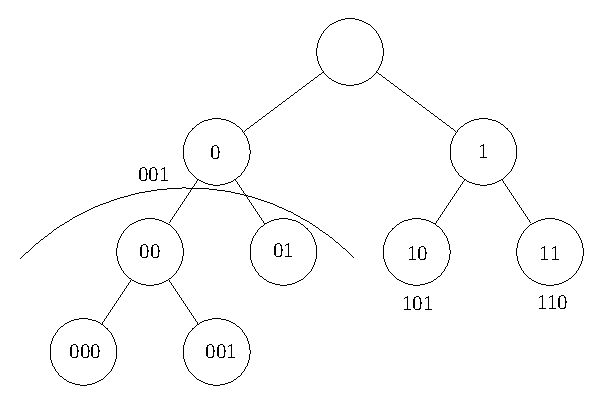
\includegraphics[width=2in]{fig3.eps}
\caption{Capture effect in 2-state QT with tag IDs \{000, 001, 101, 110\}.  The capture effect enables the reader to decode 001 when the prefix 0 is queried.  This causes the entire segment of the tree below the arc to be eliminated.  As a result, the tag with ID 000 is not singulated.  \label{fig:fig3}}
\end{figure}
In \cite{conf:Law01}, QT relies on the assumption that the tags' response to a reader query falls into one of three choices.  These are $\{$no response, one response, collision$\}$.  More precisely, the reader receiver is assumed to be able to distinguish between the three cases, and decode a tag ID only for the case of a single tag backscattering.  However, this assumption is rather strong, and ignores the capture effect.  The capture effect describes a situation where a receiver may be able to decode a signal even in the presence of other interfering signals.  In the context of QT, the reader receiver can only distinguish between two cases, namely $\{$no response, response$\}$.  If there is no response, the reader can be certain that no tags have replied.  If there is a response, the reader only knows that at least one tag has replied.  It may or may not be able to decode a tag ID from the response, but this would still not allow it to know how many tags had replied.

We call 3-state QT as the situation where no capture effect occurs.  Note that $T_{\mbox{QT}}\left(n\right)$ applies to 3-state QT.  2-state QT is when there is capture effect.  2-state QT is faulty in the sense that the reader does not necessarily singulate all $n$ tags in its range.  That is, if the capture effect causes a reader to decode a tag ID from multiple signals due to multiple tags responding to a common prefix, then all but one of those tags would not be singulated, since that segment of the query tree with that common prefix would no longer grow.  This is illustrated in Fig. \ref{fig:fig3}.  In Section \ref{sec:sims}, we show that these losses are significant.  In Section \ref{sec:gqt}, we present two simple modifications of QT that can singulate all $n$ tags, even when the capture effect is considered.

In this paper, we model the capture effect using a parameterized signal-to-interference (SIR) threshold, $\gamma$, of the reader receiver.  We assume a free space, path loss radio propagation model.  Therefore, a backscattered signal arriving at the reader has power attenuated by a factor of $d^4$, compared to the original reader transmission, where $d$ is distance between the reader and the backscattering tag.  All tags are assumed to be physically identical, and have the same effective area for absorbing incoming radio energy from the reader.  Suppose a reader query results in $l$ tags responding, where $l \in \{1, \ldots, n\}$.  Then, if the $i^{\mbox{th}}$ tag's backscatter is considered the signal, its SIR is
\begin{eqnarray}
\mbox{SIR}_i = \frac{1/d_i^4}{ \displaystyle \sum_{j \ne i, j = 1}^{l} 1/d_j^4},
\end{eqnarray}
where $d_i$ is the distance between the reader and the $i^{\mbox{th}}$ tag, and $i \in \{1, \ldots, l\}$.  If
\begin{eqnarray}
\max_{i=1}^l \mbox{SIR}_i \geq \gamma,
\end{eqnarray}
then the capture effect occurs, and the reader decodes the ID of the $k^{\mbox{th}}$ tag, where $k = \arg \max_{i=1}^l \mbox{SIR}_i$.  Therefore, $\gamma$ is a parameter that determines how effective the reader receiver is at extracting a tag ID in the midst of multiple signals.

\section{Generalized Query Tree Protocols}
\label{sec:gqt}
We introduce two modifications to QT.  Since these are natural generalizations of QT that can handle the capture effect, we call them the \em Generalized Query Tree Protocols \em (GQT1 and GQT2).  We also provide bounds on the singulation time of these two protocols, in relation to $T_{\mbox{QT}}\left(n\right)$.  In Section \ref{sec:sims}, we provide simulations to verify these results.

\subsection{GQT1}
There are two major changes that GQT1 makes to QT.  In 3-state QT, when a query prefix results in no response or a single response, we can be sure that there are no more IDs with that prefix.  In other words, this is the stopping condition of lengthening a prefix (by appending a $0$ or $1$).  However, if the capture effect is taken into consideration, a stopping condition that guarantees singulation of all tags is that there is no response.  Therefore, the first change to QT is that in GQT1, the prefix is always lengthened if there is a response.  (The one exception is if the prefix length is already $k$ bits.)  The second change is that after an ID has been decoded by the reader, it sends an ACK signal to that specific tag, to tell it to silence itself.  That is, the reader lets the tag know it has already singulated it, and the tag need not send any more backscatter responses for the rest of the singulation process.  This is important, since when the prefix is lengthened, and queried again, it may still match the ID of the previously singulated tag.  For example, suppose there are three tags with respective IDs $\{10000, 10111, 10110\}$, and the reader broadcasts a query with prefix $10$.  All three tags will respond.  Suppose the capture effect allows the reader to decode $10000$ from the three responses.  If the reader does not send an ACK signal to the first tag, and it broadcasts the next query with prefix $100$, the first tag will respond again, which is unnecessary.  This second change is also a result of the the differing stopping conditions of 3-state QT and GQT1.  GQT1 is shown below.
\begin{quote}
\begin{footnotesize}
\em GQT1 Protocol \em \\
\textbf{Reader}
\begin{enumerate}
\item $Q:=\langle0,1\rangle$, and $M:=\langle \rangle$.
\item Suppose $Q = \langle q_1, \ldots, q_l \rangle$, and \\$M = \langle t_1, \ldots, t_m\rangle$.
\item Broadcast query $q_1$ to tags.   $Q := \langle q_2, \ldots, q_l \rangle$.
\item Listen to responses from tags.
\begin{itemize}
\item If no response, then do nothing.
\item Else, try to decode a tag ID.

\begin{itemize}
\item If able to decode tag ID $t$, then \\$Q := \langle q_2, \ldots, q_l, q_10, q_11 \rangle$, and\\$M := \langle t_1, \ldots, t_m, t\rangle$. Send ACK to tag with ID $t$.
\item Else unable to decode.  \\$Q := \langle q_2, \ldots, q_l, q_10, q_11 \rangle$.
\end{itemize}

\end{itemize}
\item If $Q$ is nonempty, go to 2).
\end{enumerate}
\textbf{Tag}
\begin{enumerate}
\item Listen to query, or ACK from reader.
\begin{itemize}
\item If query prefix matches, then send tag ID.
\item Else if ACK is intended for myself, silence myself.
\end{itemize}
\item If not silenced, then go to 1).
\end{enumerate}
\end{footnotesize}
\end{quote}

GQT1 leverages the capture effect to prevent query prefixes from becoming very long, and thus, reduces the size of the query tree.  As the SIR threshold, $\gamma$, of the reader receiver increases, less ``captures" occur, and the singulation time increases.   An upper bound of $T_{\mbox{GQT1}}\left(n\right)$ is thus when $\gamma$ is sufficiently large, and therefore, the capture effect will never take place.  In this case, the algorithm runs exactly the same as QT, with the exception that there are two extra queries for each ID, since the stopping condition for GQT1 is that there is no response.  This results in an additional time of $2n$.  Recall that both a reader query and a tag response each take half a time unit.  Suppose that ACKing a tag also takes half a time unit.  Therefore, the total ACKing time is $n/2$.  We thus have the following upper bound for $n\geq2$.
\begin{eqnarray}
T_{\mbox{GQT1}}\left(n\right) \leq T_{\mbox{QT}}\left(n\right) + \frac{5}{2} n \nonumber
\end{eqnarray}
A lower bound of $T_{\mbox{GQT1}}\left(n\right)$ is when $\gamma$ is sufficiently small, and the capture effect always occurs if more than one tag responds.  In this case, the query tree will consist of a root node (which is just a place holder), $n$ other internal nodes representing the $n$ queries that each result in a decoded tag ID, and the leaves of the tree.  This is illustrated in Fig. \ref{fig:fig4}.  Since the tree is a full binary tree, we have $n+1 = r - 1$, where $r$ is the number of leaves.  Therefore, the number of nodes in the tree, excluding the root, is $n + r = 2n + 2$.  Including the total ACKing time, we have the following lower bound for $n\geq2$.
\begin{eqnarray}
T_{\mbox{GQT1}}\left(n\right) \geq 2 + \frac{5}{2} n \nonumber
\end{eqnarray}
Combining the two bounds, we have,
\begin{eqnarray}
T_{\mbox{GQT1}}\left(n\right) \in   \left[2 + \frac{5}{2} n, T_{\mbox{QT}}\left(n\right) + \frac{5}{2} n\right].
\label{eqn:t_gqt1_1}
\end{eqnarray}
Using the upper bound for $T_{\mbox{QT}}\left(n\right)$  in (\ref{eqn:t_qt}), we have
\begin{eqnarray}
T_{\mbox{GQT1}}\left(n\right) \in   \left[2 + \frac{5}{2} n, n \left( k + \frac{9}{2} - \log_2 n\right) \right].
\label{eqn:t_gqt1_2}
\end{eqnarray}
\begin{figure}
\centering
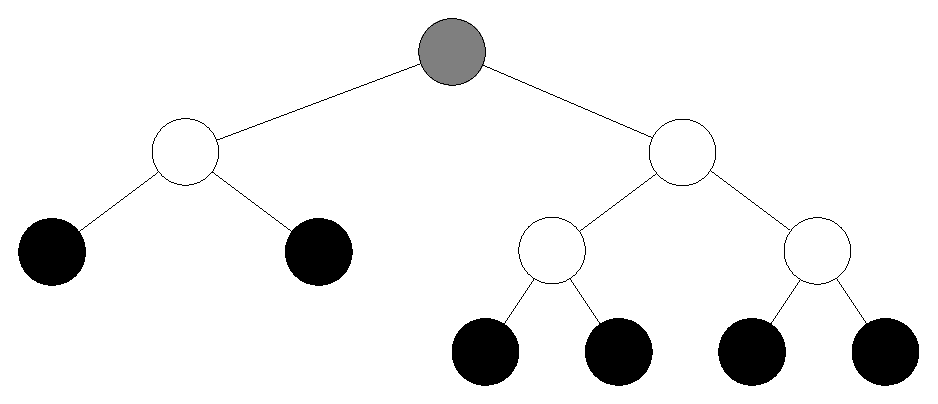
\includegraphics[width=2in]{fig4.eps}
\caption{Lower bound on $T_{\mbox{GQT1}}\left(n\right)$.  The four white internal nodes represent queries that each result in a decoded tag ID.  The six black leaf nodes represent queries that each result in no response.  We thus have, $n = 4$ and $r = 6$. \label{fig:fig4}}
\end{figure}

\subsection{GQT2}
There is only one slight change that GQT2 makes to GQT1.  To further take advantage of the capture effect, GQT2 does not append a $0$ or $1$ to the prefix when the reader decodes a tag ID.  Rather, the reader re-broadcasts the same prefix.  Since the ACK silences the tag that was just singulated in the previous query, another tag can be ``captured" using the same prefix.  Only when no ID can be decoded from a response does the reader append $0$ or $1$ to the prefix.  GQT2 is shown below.
\begin{quote}
\begin{footnotesize}
\em GQT2 Protocol \em \\
\textbf{Reader}
\begin{enumerate}
\item $Q:=\langle0,1\rangle$, and $M:=\langle \rangle$.
\item Suppose $Q = \langle q_1, \ldots, q_l \rangle$, and \\$M = \langle t_1, \ldots, t_m\rangle$.
\item Broadcast query $q_1$ to tags.   $Q := \langle q_2, \ldots, q_l \rangle$.
\item Listen to responses from tags.
\begin{itemize}
\item If no response, then do nothing.
\item Else, try to decode a tag ID.

\begin{itemize}
\item If able to decode tag ID $t$, then \\$Q := \langle q_2, \ldots, q_l, q_1 \rangle$, and \\$M := \langle t_1, \ldots, t_m, t\rangle$. Send ACK to tag with ID $t$.
\item Else unable to decode.  \\$Q := \langle q_2, \ldots, q_l, q_10, q_11 \rangle$.
\end{itemize}

\end{itemize}
\item If $Q$ is nonempty, go to 2).
\end{enumerate}
\textbf{Tag}
\begin{enumerate}
\item Listen to query, or ACK from reader.
\begin{itemize}
\item If query prefix matches, then send tag ID.
\item Else if ACK is intended for myself, silence myself.
\end{itemize}
\item If not silenced, then go to 1).
\end{enumerate}
\end{footnotesize}
\end{quote}

An upper bound of $T_{\mbox{GQT2}}\left(n\right)$ follows the same reasoning of the upper bound of  $T_{\mbox{GQT1}}\left(n\right)$.  The only difference is that there is only one extra query for each ID, since after decoding a tag ID from a prefix, it only has to re-broadcast the same prefix to detect that there is no response, which is the stopping condition.  The upper bound for $n\geq2$ is thus,
\begin{eqnarray}
T_{\mbox{GQT2}}\left(n\right) \leq T_{\mbox{QT}}\left(n\right) + \frac{3}{2} n \nonumber
\end{eqnarray}
A lower bound of $T_{\mbox{GQT1}}\left(n\right)$ is when $\gamma$ is sufficiently small, and the capture effect always occurs if more than one tag responds.  In this case, the initial prefixes $\{0, 1\}$ are sufficient to decode all the IDs, one-by-one with the capture effect.  This contributes a time of $n$.  There are also two extra queries, one for each prefix that results in the stopping condition.  Including the total ACKing time, the lower bound for $n\geq2$ is thus,
\begin{eqnarray}
T_{\mbox{GQT2}}\left(n\right) \geq 2 + \frac{3}{2} n \nonumber
\end{eqnarray}
Combining the two bounds, we have,
\begin{eqnarray}
T_{\mbox{GQT2}}\left(n\right) \in   \left[2 + \frac{3}{2} n, T_{\mbox{QT}}\left(n\right) + \frac{3}{2} n\right].
\label{eqn:t_gqt2_1}
\end{eqnarray}
Using the upper bound for $T_{\mbox{QT}}\left(n\right)$  in (\ref{eqn:t_qt}), we have
\begin{eqnarray}
T_{\mbox{GQT2}}\left(n\right) \in   \left[2 + \frac{3}{2} n, n \left( k + \frac{7}{2} - \log_2 n\right) \right].
\label{eqn:t_gqt2_2}
\end{eqnarray}

\section{Simulation Results}
\label{sec:sims}
We present Monte Carlo simulation results of the three protocols described in this paper.  All results are averages.  In all cases, $k=12$ bits is chosen to be the length of a tag ID.  $n = 10, 20, \ldots, 100$ is the number of tags within the range of the reader.  The tag IDs are unique and chosen from a uniform distribution.  For the  2-state QT, GQT1 and GQT2 cases, the locations of the tags in the unit disk are also chosen from a uniform distribution.  The tag distances are used to calculate when the capture effect occurs using the parameterized SIR threshold, $\gamma$.

\subsection{QT}
Fig. \ref{fig:fig5a} shows the average singulation time of 3-state QT, i.e. $T_{\mbox{QT}}\left(n\right)$. \cite{conf:Law01} says that $T_{\mbox{QT}}\left(n\right)$ is $O\left(n\right)$ with high probability.  The straight line confirms this.  The upper bound in (\ref{eqn:t_qt}) is also shown, which appears very loose.  Fig. \ref{fig:fig5b} shows the number of tags that 2-state QT fails to singulate, due to the capture effect.  The plot shows that the percentage of missed tags stays fairly stable as $n$ is increased.  As $\gamma$ is decreased, the capture effect becomes more pronounced (i.e. more ``captures" occur), and thus, more tags are not singulated.  For $\gamma = 5$ dB, and $n=100, 78$ tags are not singulated.

\subsection{GQT1, GQT2}
Fig. \ref{fig:fig6a} and Fig. \ref{fig:fig6b} show the average singulation times of GQT1 and GQT2, i.e. $T_{\mbox{GQT1}}\left(n\right)$ and $T_{\mbox{GQT2}}\left(n\right)$, respectively.  The upper and lower bounds in (\ref{eqn:t_gqt1_1}) and (\ref{eqn:t_gqt2_1}) are also shown respectively, in the two plots.  As expected, as $\gamma$ increases, there are less ``captures", and the average singulation time increases.  In both protocols, $\gamma = 100$ dB is sufficient for the average singulation time to approximate the upper bound, and $\gamma = -5$ dB for the lower bound.  Fig. \ref{fig:fig7} compares the average singulation times of 3-state QT, GQT1 and GQT2.  3-state gives the best performance (since the capture effect is ignored in this case).  GQT2 performs better than GQT1 at the same $\gamma$.  At $\gamma = 5$ dB and $n=100$, GQT2 requires approximately $66$ additional seconds compared to 3-state QT.

\section{Conclusion}
\label{sec:con}
QT is an efficient RFID tag singulation algorithm.  However, it ignores the capture effect.  In this paper, we provide GQT1 and GQT2, two natural generalizations of QT that retain the tree-based spirit of QT, but also cope with the capture effect.  Analytic bounds, and simulation results of the singulation times of these protocols are also provided.

\begin{figure*}
\centerline{
    \subfigure[Average singulation time of 3-state QT.]{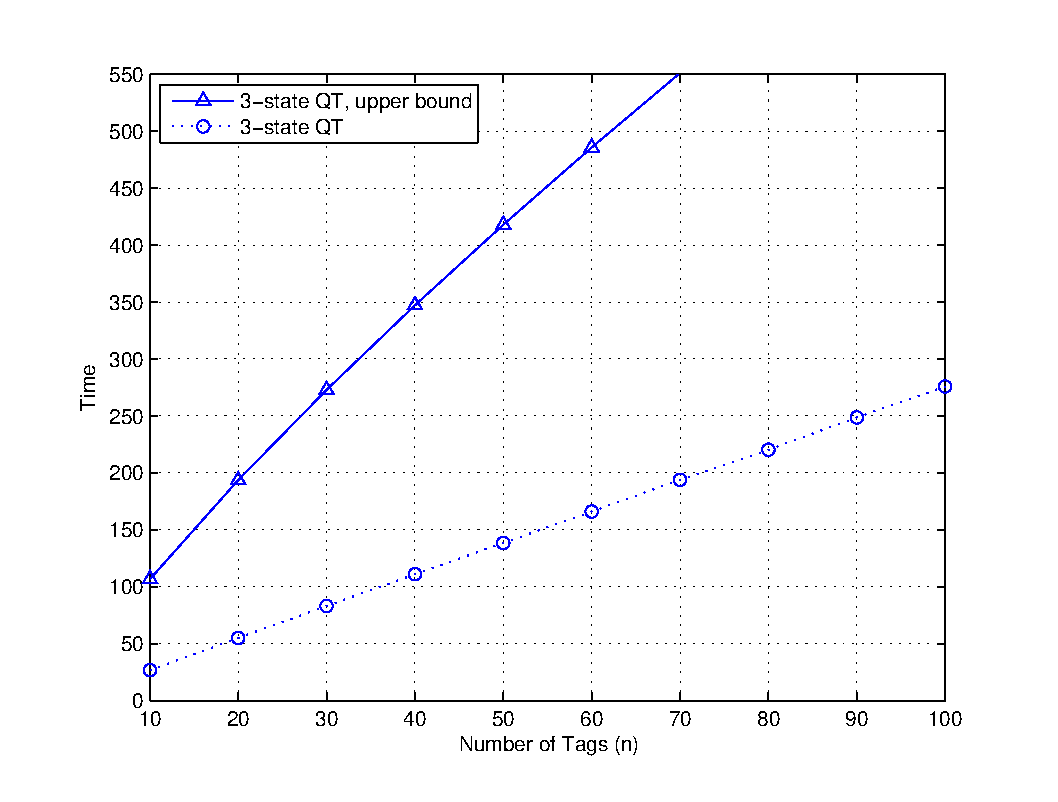
\includegraphics[width=3.25in]{fig5a.eps} \label{fig:fig5a}}
    \subfigure[Average number of unsingulated tags in 2-state QT.]{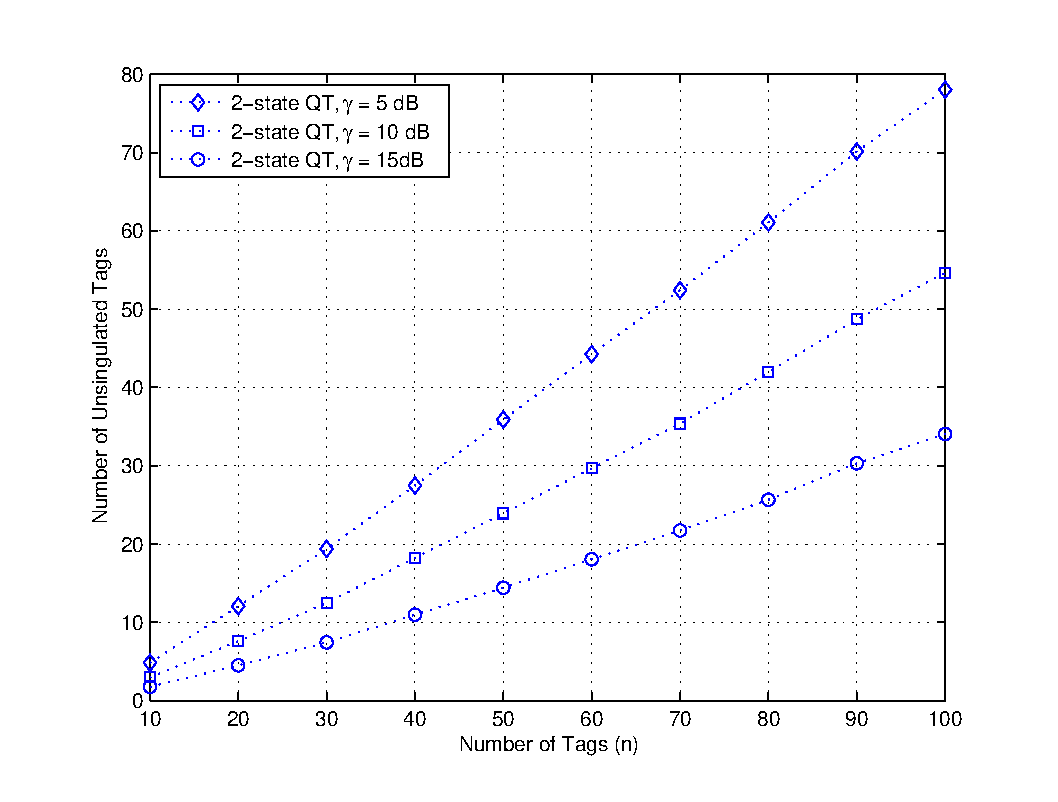
\includegraphics[width=3.25in]{fig5b.eps} \label{fig:fig5b}} \\
}
 \caption{QT simulation results.}
\label{}
\end{figure*}
\begin{figure*}
\centerline{
    \subfigure[Average singulation time of GQT1.]{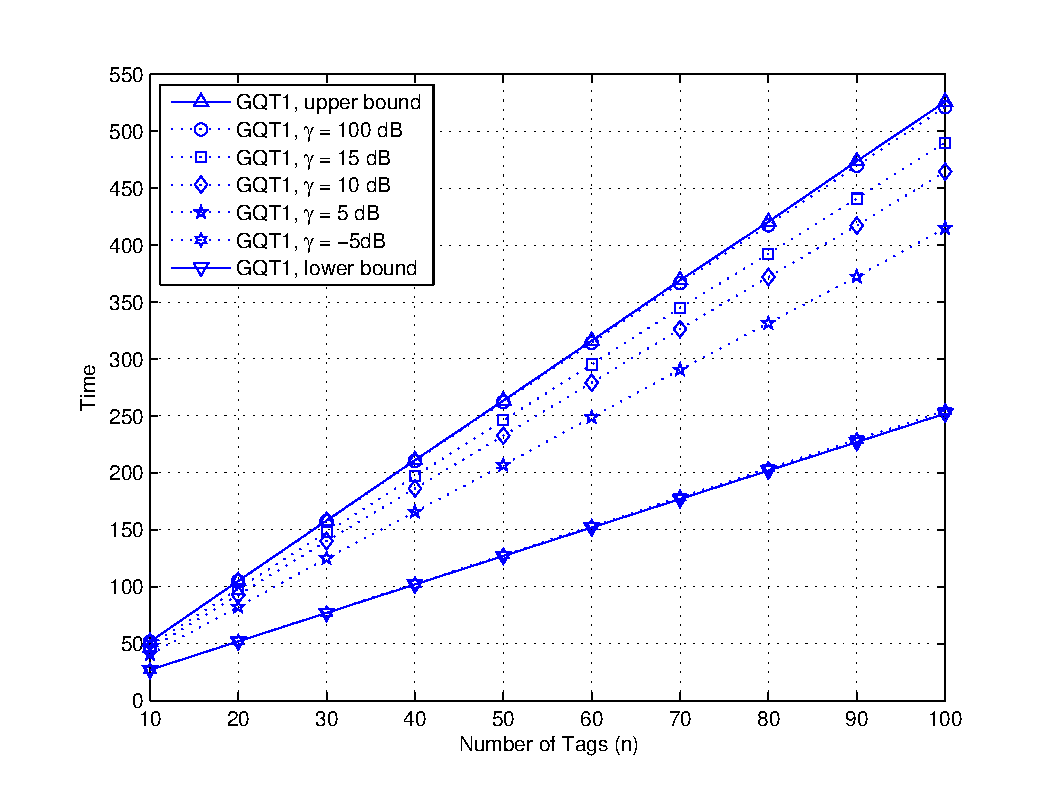
\includegraphics[width=3.25in]{fig6a.eps} \label{fig:fig6a}}
    \subfigure[Average singulation time of GQT2.]{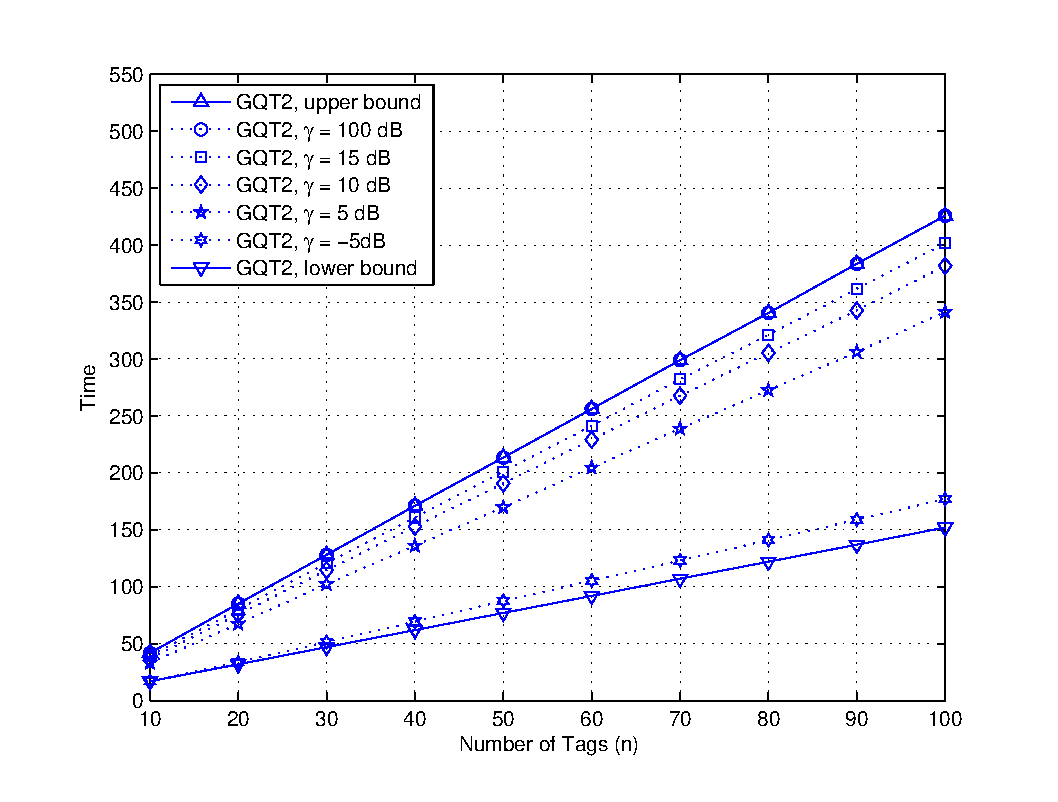
\includegraphics[width=3.25in]{fig6b.eps} \label{fig:fig6b}} \\
}
 \caption{GQT1, GQT2 simulation results.}
\label{}
\end{figure*}

\begin{figure}
\centering
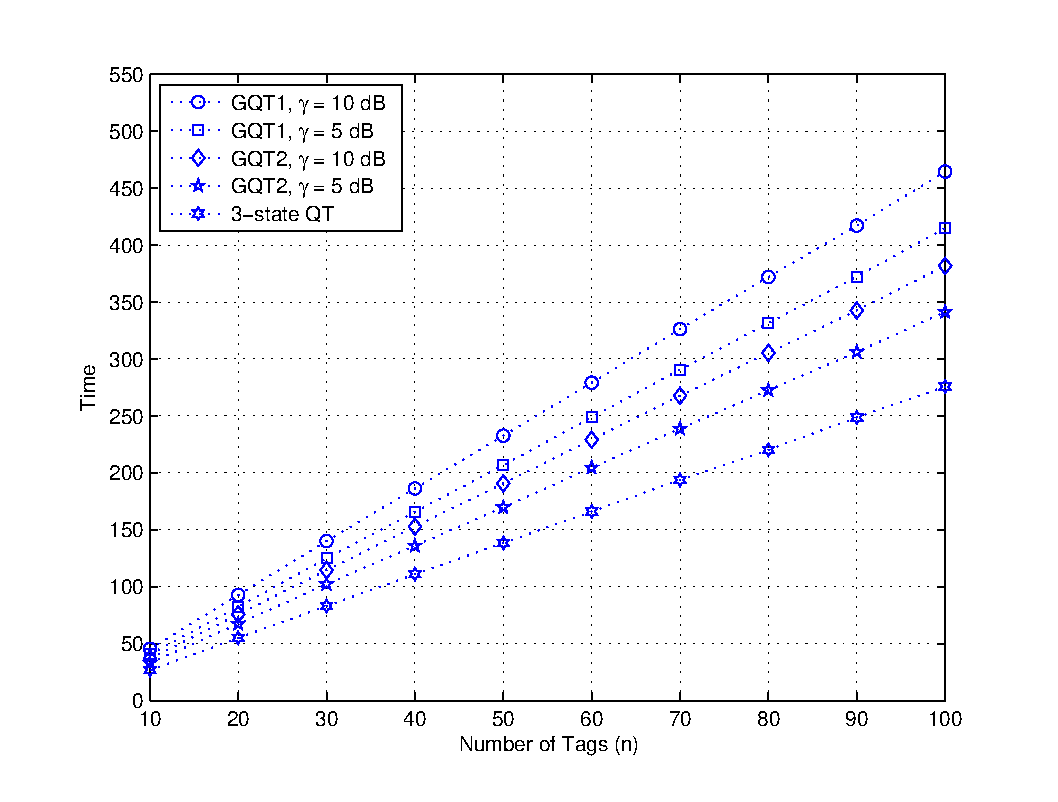
\includegraphics[width=3.25in]{fig7.eps}
\caption{Average singulation time comparison of 3-state QT, GQT1 and GQT2.  \label{fig:fig7}}
\end{figure}

% An example of a floating figure using the graphicx package.
% Note that \label must occur AFTER (or within) \caption.
% For figures, \caption should occur after the \includegraphics.
% Note that IEEEtran v1.7 and later has special internal code that
% is designed to preserve the operation of \label within \caption
% even when the captionsoff option is in effect. However, because
% of issues like this, it may be the safest practice to put all your
% \label just after \caption rather than within \caption{}.
%
% Reminder: the "draftcls" or "draftclsnofoot", not "draft", class
% option should be used if it is desired that the figures are to be
% displayed while in draft mode.
%
%\begin{figure}[!t]
%\centering
%\includegraphics[width=2.5in]{myfigure}
% where an .eps filename suffix will be assumed under latex,
% and a .pdf suffix will be assumed for pdflatex; or what has been declared
% via \DeclareGraphicsExtensions.
%\caption{Simulation Results}
%\label{fig_sim}
%\end{figure}

% Note that IEEE typically puts floats only at the top, even when this
% results in a large percentage of a column being occupied by floats.


% An example of a double column floating figure using two subfigures.
% (The subfig.sty package must be loaded for this to work.)
% The subfigure \label commands are set within each subfloat command, the
% \label for the overall figure must come after \caption.
% \hfil must be used as a separator to get equal spacing.
% The subfigure.sty package works much the same way, except \subfigure is
% used instead of \subfloat.
%
%\begin{figure*}[!t]
%\centerline{\subfloat[Case I]\includegraphics[width=2.5in]{subfigcase1}%
%\label{fig_first_case}}
%\hfil
%\subfloat[Case II]{\includegraphics[width=2.5in]{subfigcase2}%
%\label{fig_second_case}}}
%\caption{Simulation results}
%\label{fig_sim}
%\end{figure*}
%
% Note that often IEEE papers with subfigures do not employ subfigure
% captions (using the optional argument to \subfloat), but instead will
% reference/describe all of them (a), (b), etc., within the main caption.


% An example of a floating table. Note that, for IEEE style tables, the
% \caption command should come BEFORE the table. Table text will default to
% \footnotesize as IEEE normally uses this smaller font for tables.
% The \label must come after \caption as always.
%
%\begin{table}[!t]
%% increase table row spacing, adjust to taste
%\renewcommand{\arraystretch}{1.3}
% if using array.sty, it might be a good idea to tweak the value of
% \extrarowheight as needed to properly center the text within the cells
%\caption{An Example of a Table}
%\label{table_example}
%\centering
%% Some packages, such as MDW tools, offer better commands for making tables
%% than the plain LaTeX2e tabular which is used here.
%\begin{tabular}{|c||c|}
%\hline
%One & Two\\
%\hline
%Three & Four\\
%\hline
%\end{tabular}
%\end{table}


% Note that IEEE does not put floats in the very first column - or typically
% anywhere on the first page for that matter. Also, in-text middle ("here")
% positioning is not used. Most IEEE journals/conferences use top floats
% exclusively. Note that, LaTeX2e, unlike IEEE journals/conferences, places
% footnotes above bottom floats. This can be corrected via the \fnbelowfloat
% command of the stfloats package.







% trigger a \newpage just before the given reference
% number - used to balance the columns on the last page
% adjust value as needed - may need to be readjusted if
% the document is modified later
%\IEEEtriggeratref{8}
% The "triggered" command can be changed if desired:
%\IEEEtriggercmd{\enlargethispage{-5in}}

% references section

% can use a bibliography generated by BibTeX as a .bbl file
% BibTeX documentation can be easily obtained at:
% http://www.ctan.org/tex-archive/biblio/bibtex/contrib/doc/
% The IEEEtran BibTeX style support page is at:
% http://www.michaelshell.org/tex/ieeetran/bibtex/
%\bibliographystyle{IEEEtran}
% argument is your BibTeX string definitions and bibliography database(s)
%\bibliography{IEEEabrv,../bib/paper}
%
% <OR> manually copy in the resultant .bbl file
% set second argument of \begin to the number of references
% (used to reserve space for the reference number labels box)
\bibliographystyle{IEEEtran}
% argument is your BibTeX string definitions and bibliography database(s)
\bibliography{IEEEabrv,IEEEexample}






% that's all folks
\end{document}


